%%%%%%%%%%%%%%%%%%%%%%%%%%%%%%%%%%%%%%%%%
% Beamer Presentation LaTeX Template Version 1.0 (10/11/12)
%
% This template has been downloaded from:
% http://www.LaTeXTemplates.com
%
% License: CC BY-NC-SA 3.0
% (http://creativecommons.org/licenses/by-nc-sa/3.0/)
%
%%%%%%%%%%%%%%%%%%%%%%%%%%%%%%%%%%%%%%%%%

% ----------------------------------------------------------------------------------------
% PACKAGES AND THEMES
% ----------------------------------------------------------------------------------------

\documentclass{beamer}

\mode<presentation> {

  % The Beamer class comes with a number of default slide themes which
  % change the colors and layouts of slides. Below this is a list of
  % all the themes, uncomment each in turn to see what they look like.

  % \usetheme{default} \usetheme{AnnArbor} \usetheme{Antibes}
  % \usetheme{Bergen} \usetheme{Berkeley} \usetheme{Berlin}
  % \usetheme{Boadilla} \usetheme{CambridgeUS} \usetheme{Copenhagen}
  % \usetheme{Darmstadt} \usetheme{Dresden} \usetheme{Frankfurt}
  % \usetheme{Goettingen} \usetheme{Hannover} \usetheme{Ilmenau}
  % \usetheme{JuanLesPins} \usetheme{Luebeck}
  \usetheme{Madrid}
  % \usetheme{Malmoe} \usetheme{Marburg} \usetheme{Montpellier}
  % \usetheme{PaloAlto} \usetheme{Pittsburgh} \usetheme{Rochester}
  % \usetheme{Singapore} \usetheme{Szeged} \usetheme{Warsaw}

  % As well as themes, the Beamer class has a number of color themes
  % for any slide theme. Uncomment each of these in turn to see how it
  % changes the colors of your current slide theme.

  % \usecolortheme{albatross}
  \usecolortheme{beaver}
  % \usecolortheme{beetle} \usecolortheme{crane}
  % \usecolortheme{dolphin} \usecolortheme{dove} \usecolortheme{fly}
  % \usecolortheme{lily} \usecolortheme{orchid} \usecolortheme{rose}
  % \usecolortheme{seagull} \usecolortheme{seahorse}
  % \usecolortheme{whale} \usecolortheme{wolverine}

  % \setbeamertemplate{footline} % To remove the footer line in all slides uncomment this line
  % \setbeamertemplate{footline}[page
  % number] % To replace the footer line in all slides with a simple slide count uncomment this line

  % \setbeamertemplate{navigation
  % symbols}{} % To remove the navigation symbols from the bottom of all slides uncomment this line
}
% xtong's tools
% aliasis
\newcommand{\xemp}[1]{{\color{red}{\textbf{#1}}}}
\newcommand{\bs}{\boldsymbol}
\newcommand{\mean}[2]{\left\langle{#1}\right\rangle_{#2}}
\newcommand{\trb}[1]{\textrm{Tr}\left({#1}\right)}
\newcommand{\trs}[1]{\textrm{Tr}\left[{#1}\right]}
\newcommand{\invb}[1]{{\left({#1}\right)^-}}
\newcommand{\invs}[1]{{\left[{#1}\right]^-}}
\newcommand\numberthis{\addtocounter{equation}{1}\tag{\theequation}}
\renewcommand{\eqref}[1]{Eq.\,\ref{#1}}
%
% vectors and matrices
\newcommand{\va}{\mathbf{a}}
\newcommand{\vb}{\mathbf{b}}
\newcommand{\vc}{\mathbf{c}}
\newcommand{\vf}{\mathbf{f}}
\newcommand{\vg}{\mathbf{g}}
\newcommand{\vh}{\mathbf{h}}
\newcommand{\vv}{\mathbf{v}}
\newcommand{\vx}{\mathbf{x}}
\newcommand{\vu}{\mathbf{u}}
\newcommand{\vy}{\mathbf{y}}
\newcommand{\vw}{\mathbf{w}}
\newcommand{\vs}{\mathbf{s}}
% 
\newcommand{\xf}{\mathbf{F}}
\newcommand{\xg}{\mathbf{G}}
\newcommand{\xh}{\mathbf{H}}
\newcommand{\xk}{\mathbf{K}}
\newcommand{\xl}{\mathbf{L}}
\newcommand{\xr}{\mathbf{R}}
%
\newcommand{\xu}{\mathbf{U}}
\newcommand{\xv}{\mathbf{V}}
\newcommand{\xx}{\mathbf{X}}
\newcommand{\xw}{\mathbf{W}}
\newcommand{\xy}{\mathbf{Y}}
\newcommand{\xz}{\mathbf{Z}}
\newcommand{\xa}{\mathbf{A}}
\newcommand{\xd}{\mathbf{D}}
% 
% with tildes
%% vectors
\newcommand{\vat}{\tilde{\vb}}
\newcommand{\vbt}{\tilde{\vb}}
\newcommand{\vct}{\tilde{\vc}}
\newcommand{\vht}{\tilde{\vh}}
\newcommand{\vvt}{\tilde{\vv}}
\newcommand{\vst}{\tilde{\vs}}
\newcommand{\vut}{\tilde{\vu}}
\newcommand{\vft}{\tilde{\vf}}
\newcommand{\xut}{\tilde{\xu}}
\newcommand{\vxt}{\tilde{\vx}}
\newcommand{\xvt}{\tilde{\xv}}
\newcommand{\xyt}{\tilde{\xy}}
%% matrices
\newcommand{\xwt}{\tilde{\xw}}
%
% with hats
\newcommand{\vhh}{\hat{\vh}}
\newcommand{\xvh}{\hat{\xv}}
\newcommand{\vvh}{\hat{\vv}}
\newcommand{\vyh}{\hat{\vy}}
\newcommand{\vxh}{\hat{\vx}}
\newcommand{\vuh}{\hat{\vu}}
\newcommand{\vfh}{\hat{\vf}}
\newcommand{\xyh}{\hat{\xy}}
\newcommand{\xxh}{\hat{\xx}}
\newcommand{\xuh}{\hat{\xu}}
%
%
% derivatives
\newcommand{\DRV}[2]{\frac{d #1}{d #2}}
\newcommand{\DRC}[3]{\DRV{#1}{#2}\DRV{#2}{#3}}
\newcommand{\PDV}[2]{\frac{\partial #1}{\partial #2}}
\newcommand{\PDC}[3]{\PDV{#1}{#2}\PDV{#2}{#3}}
%
% the diagnal matrix
\newcommand{\id}{\textrm{\textbf{I}}}
\newcommand{\im}{\textrm{\textbf{I}}}
% the vector of ones
\newcommand{\one}{\mathbf{1}}
% 
% xiaoran's edit
\newcommand{\xadd}[1]{\textcolor{blue}{#1}}
\newcommand{\xdel}[1]{\textcolor{red}{\sout{#1}}}
\newcommand{\xrpl}[2]{\xdel{#1}\xadd{#2}}
\newcommand{\xacc}[1]{\textcolor{ForestGreen}{#1}}
%
%
% declarations
% argument of the minimum / maximum
\DeclareMathOperator*{\argmin}{arg\,min}
\DeclareMathOperator*{\argmax}{arg\,max}
%
% norms
\newcommand\norm[1]{\left\lVert#1\right\rVert}
\newcommand{\xmx}{\bs{X}} \newcommand{\xmt}{\bs{X}^{\prime}}
\newcommand{\imx}{\bs{I}} \newcommand{\umx}{\bs{U}}
\newcommand{\umt}{\bs{U}^{\prime}} \newcommand{\yvc}{\bs{y}}
\newcommand{\yht}{\hat{\bs{y}}}
\usepackage{graphicx} % Allows including images
\usepackage{booktabs} % Allows the use of \toprule, \midrule and \bottomrule in tables

% ----------------------------------------------------------------------------------------
% TITLE PAGE
% ----------------------------------------------------------------------------------------

\title[Kernel Genomics]{Meta analysis of Variance Components \\
  simulation study}

\author{Xiaoran Tong} % Your name
\institute[EPI Biosta,
MSU] % Your institution as it will appear on the bottom of every slide, may be shorthand to save space
{ Michigan State University \\ % Your institution for the title page
  \medskip \textit{tongxia1@msu.edu} \\% Your email address
  \textit{qlu@epi.msu.edu} % Your email address
} \date{\today} % Date, can be changed to a custom date

\begin{document}

\begin{frame}
  \titlepage % Print the title page as the first slide
\end{frame}

\begin{frame}
  \frametitle{Table of
    Content} % Table of contents slide, comment this block out to remove it
  \tableofcontents % Throughout your presentation, if you choose to use \section{} and \subsection{} commands, these will automatically be printed on this slide as an overview of your presentation
\end{frame}

% ----------------------------------------------------------------------------------------
% PRESENTATION SLIDES
% ----------------------------------------------------------------------------------------
\section{Introduction}
% ----------------------------------------------------------------------------------------
\begin{frame}
  \frametitle{Introduction} %
  \textbf{Variance Component Model (VCM):} \\
  are suitable to depict the influence of ultra high dimentional $\xx$
  on $\vy$, with an typical construct of
  \begin{align}\label{eq:vcm}
    h(\vy) \sim \mathcal{N}(0, \xv), \quad
    \xv = \xv_{\bs{e}} + \xv_{\xx} = \sigma^2_0 \id + \sum_{i=1}^L
    \sigma^2_i \mathcal{K}_i(\xx)
  \end{align}
  \begin{itemize}
  \item $h$ transform $\vy$ into a sample from multivariate normrl of
    mean $\bs{0}^N$ and covariance $\xv^{N \times N}$;
  \item $\xv$ is determined partially by $\xx$ through $L$ kernels:
    $\{\mathcal{K}_{1 \dots L}\}$, while the rest is left to an white
    kernel $\id$;
  \item kernels are weighted by the to be fitted \textbf{variance
      component (VC)}
    $\bs{\theta} = \{\sigma^2_0, \sigma^2_1 \dots \sigma^2_L\}$.
  \end{itemize}
\end{frame}
% ----------------------------------------------------------------------------------------
\begin{frame}
  \textbf{Motivation of Meta-analysis by VCM (MVCM)}: \\
  One would like to applay meta-analys to a number of variance
  component models because
  \begin{itemize}
  \item VCM is one way to exam the overall effect of $P$ variable on
    $\vy$;
  \item VCM dealt with the dimensionality issue by encoding the
    $N \times P$ data with a few kernels of size $N \times N$.
  \item meta-analysis helps to
    \begin{itemize}
    \item pool a huge sample required to fit a VCM
    \item distribute the computational, logistical, and financial
      burderns.
    \end{itemize}
  \end{itemize}
\end{frame}
% ----------------------------------------------------------------------------------------
\begin{frame}
  \textbf{Issues of VCM}
  \begin{itemize}
  \item computation remains to be a issue due to matrix inversion
    involed
  \item the status-quo construct (\ref{eq:vcm}) is under powered when
    faced with weak and non-linear effects.
  \item logistic issues remains:
    \begin{itemize}
    \item kernels are not suitible to store in a meta-analysis server
    \item kernels can be used to triangulate individuals by group;
    \end{itemize}
  \end{itemize}
\end{frame}
% ----------------------------------------------------------------------------------------
\section{Simulations}
\begin{frame}
  \frametitle{Simulation Settings:} \textbf{Genomic Data Source
    $\xg$:}
  \begin{itemize}
  \item Drawn from 1000 Genome Project (total sample size is 2504);
  \item $P=3000$ SNP (MAF $> 0.01$) from a segment of chrosome 3.
  \item $N=500$ per cohort;
  \item $Q=4$ developing cohorts, $R=1$ evaluation cohort;
  \end{itemize}
  \textbf{Functional variants $\xx$:}
  \begin{itemize}
  \item $f = 0.1$, the fraction of functional SNPs;
  \item $\xx = (\one\vm^T) \odot \xg, \quad \vm \sim \mathcal{B}^P(f)$
  \item $\xx$ is the function part of genome data $\xg$
  \item $\vm$ is a vector mask of funtional variants
  \item $\mathcal{B}^P(f)$: $P$ Bernoulli experiments of success rate
    $f$.
  \end{itemize}
\end{frame}
% ---------------------------------------------------------
\begin{frame}
  \frametitle{Simulation Settings:}%
  \textbf{Response Generation: homogeneous effect}
  \begin{itemize}
  \item
    $ \vz_h \sim \mathcal{N}(\bs{0}, \sigma^2_0 \id + \sum_{i=1}^L
    \sigma_i^2 \mathcal{K}_i(\xx))$
  \item up to 3 kernels built from $\xx$:
    \begin{itemize}
    \item Normalized Gaussian:
      \begin{align}
        k(\vx, \vx^\prime)= \exp{[\frac{1}{2Pf}{\norm{\vx, \vx^\prime}_2^2}]}
      \end{align}
    \item Normalized Polynomial up to the 2nd order:
      \begin{align}
        \mathcal{K}(\xx, q)=(\frac{1}{Pf}\xx\xx^T)^q, \quad q={1, 2}
      \end{align}
    \end{itemize}
  \item variance components:
    \begin{align*}
      \sigma_0^2 = 0.1; \quad \sigma^2_i \sim \chi^2_2, \quad i = 1 \dots L
    \end{align*}
  \end{itemize}
\end{frame}
% ---------------------------------------------------------
\begin{frame}
  \frametitle{Simulation Settings:} %
  \textbf{Response Generation: heterogeneous effect}:\\
  \begin{itemize}
  \item the variance components varies across the $Q$ cohorts.
  \item the white noise and type of kernel is unchanged
    \begin{align*}
      \vz_j & \sim \mathcal{N}(\bs{0}, \sigma^2_0 \id + \sum_{i=1}^L
              \sigma_{i,j}^2 \mathcal{K}_i(\xx_j)), \quad
              \sigma_{i,j}^2 \sim \chi_2^2, \quad
              j = 1 \dots Q
    \end{align*}
  \item the total effect $\vz$ is a mix between the homogeneous and
    the cohort specifit heterogeneous effect.
  \end{itemize}
  \begin{align*}
    \vz & = \vz_h (1-\alpha) + [\vz_1^T, \dots, \vz_Q^T]^T \alpha,
          \quad \alpha \in [0, 1]
  \end{align*}
  Gradually increase the ratio of heterogeneity $alpha$ from 0 (fully
  homogeneous) to 1 (fully heterogeneous).
\end{frame}
\begin{frame}
  Generating heterogeneous effect:
  \begin{figure}
    \centering
    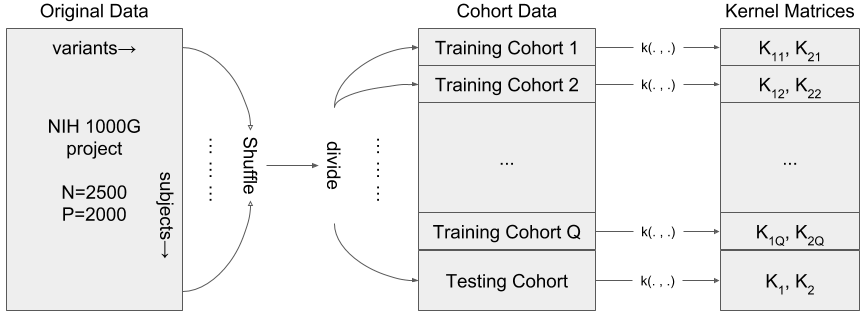
\includegraphics[width=\linewidth]{kma_sim_1kg.png}
  \end{figure}
\end{frame}
% ---------------------------------------------------------
\begin{frame}
  \frametitle{Simulation Settings:} %
  \textbf{Response Generation: Transformation on $\vy$:}
  \begin{itemize}
  \item the inverse transformation $g=h^{-1}$ is applied:
    $\vy=g(\vz)$.
  \item $g$ can be a distribution morph:
    \begin{itemize}
    \item normal $\bs{z}$ morph to student $t_{10}$ for outliers;
    \item normal $\bs{z}$ morph to $\mathcal{B}(p)$ for discretion;
    \end{itemize}
    derive the probability $p_*$ of $z_*$ either empirically, or from
    the diagnal of combined covariance; \\
    search $p_*$ in the quantile table of the target distribution for
    morphed value $y_*$;
  \item $g$ can also be a direct transform, for example:
    $$ y_* = \mathtt{sigmoid}(z_*), \quad \mathtt{or} \quad y_* = \mathtt{sin}(2\pi z_*) $$
  \end{itemize}
\end{frame}
% ---------------------------------------------------------% ---------------------------------------------------------
\begin{frame}
  \frametitle{Simulation Settings:} %
  \textbf{Training:}
  \begin{itemize}
  \item working model: normalized polynomial up to the 2nd order built
    from all variants $\xg$
    \begin{align}\label{eq:dvp}
      \xvh = \xvh_e + \xvh_\xg = \hat{\sigma}^2_0\id +
      \hat{\sigma}_1^2 (\frac{1}{P}{\xg \xg^T}) + \hat{\sigma}_2^2
      (\frac{1}{P}{\xg \xg^T})^2
    \end{align}
  \item for each cohort, use non-batched MINQUE for simplicity;
  \item pooling strategies:
    \begin{itemize}
    \item meta-analysis: aggregation of $Q$ sub-models
    \item mega-analysis: one model derived from the entire
      $N \times Q$ data
    \item average analyse: apply each sub-model to the testing data,
      get average performance, this is actually a non-pooling, but
      included for benchmark purpose.
    \end{itemize}
  \end{itemize}
\end{frame}
% ---------------------------------------------------------
\begin{frame}
  \frametitle{Simulation Settings:} %
  \textbf{Testing Performance} \\
  Let $(\vy, \xg)$ denote the testing cohort. First make a prediction
  of $\vyh$ assuming it is normal, even for MINQUE:
  \begin{align}
    \begin{split}
      \vyh &= \xvh_\xg \xvh^{-1} \vy,
    \end{split}
  \end{align}
  where $\xvh_\xg$ and $\xvh$ take the same form of (\ref{eq:dvp}).\\
  \textbf{Use the following performance criteria}
  \begin{itemize}
  \item $\mathtt{MSE} = \frac{1}{N} \norm{\vy, \hat{\vy}}_2^2 = \frac{1}{N} (\vy-\vyh)^T(\vy-\vyh)$
  \item
    $\mathtt{MNL} = \frac{1}{N} [\frac{1}{2}\vy\xvh^{-1}\vy +
    \frac{1}{2}\log{|\xvh|} + \frac{N}{2}\log{2\pi}]$
  \end{itemize}
\end{frame}
%---------------------------------------------------------
\section{Simulation Results}
% ---------------------------------------------------------
\begin{frame}{EXP 01: Use MINQUE, NLK plotted}
  \scriptsize super plot, left to right: gradual increase of heterogeneity;\\
  top: response is normal; bottom: response morphed into $t_{10}$ \\
  \normalsize
  \begin{figure}
    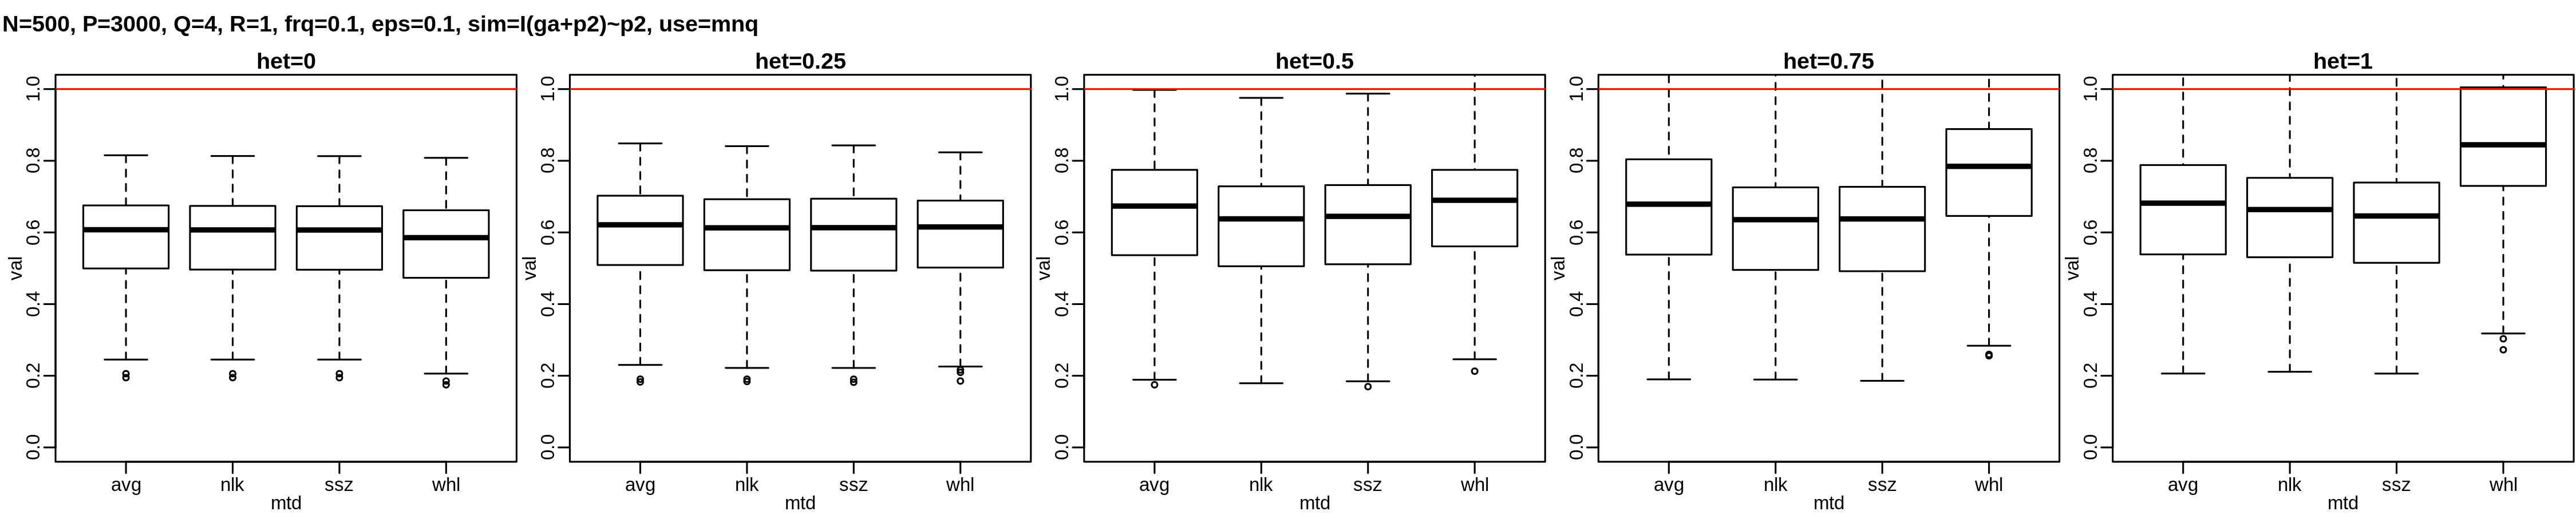
\includegraphics[width=\linewidth]{km2_mnq_s01.png} \\
    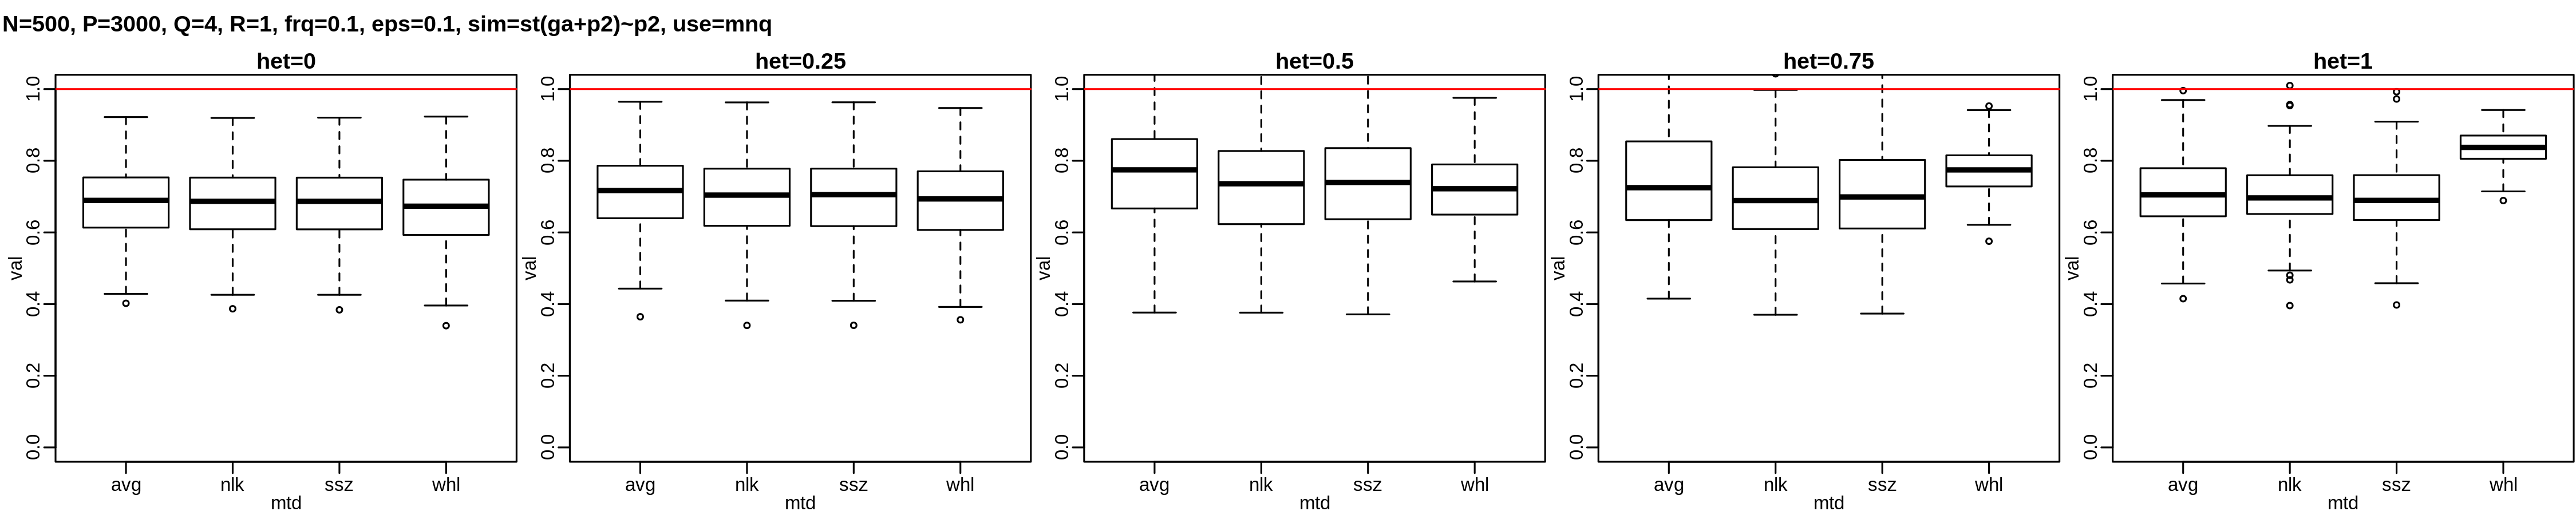
\includegraphics[width=\linewidth]{km2_mnq_s02.png}
  \end{figure}
  \tiny sub plot, left to right, avg: average performance without pooling;\\
  nlk and ssz: meta-analysis, model pooled by liklihood or sample size; \\
  whl: mega-analysis, model trained from the whole sample;
\end{frame}
% ---------------------------------------------------------
\section{Speculation}
\begin{frame}
  \frametitle{Speculation}
  \begin{itemize}
  \item increased inter-cohort heterogeneity cost the generalization
    of models built from mega-analyis.
  \item meta-analysis is robust to such heterogeneity.
  \item mana-analysis only suits for fully homogeneous populations.
  \item even without pooling of models (meta) or data (mega), the
    averge performance of sub-models are almost stable across levels
    of heterogeneity, showing the effect of a bagging assemble.
  \end{itemize}
\end{frame}
% ---------------------------------------------------------
\end{document}
